%!TEX root = geometry.tex
\stepcounter{lecture}
\setcounter{lecture}{1}
\sektion{Euclidean geometry}

\subsection[Geometry in $\Rn$]{Geometry in $\boldsymbol{\sf{R}^\sf{n}}$} % (fold)
\label{sub:geometry_in_rn}

\lecturemarker{1}{21 Jan}

For $\vv, \ww \iRn$, the \emph{dot product} is defined as
\begin{equation*}
	\vv \cdot \ww = \sum_{i=1}^n v_i \, w_i.
\end{equation*}
The \emph{norm} or ``length'' of a vector is
\begin{equation*}
	\left\vert \vv \right\vert = \sqrt{\vv \cdot \vv}
\end{equation*}
and this satisfies the triangle inequality:
\begin{equation*}
	\left\vert \vv + \ww \right\vert \leq \left\vert \vv \right\vert + \left\vert \ww \right\vert,
\end{equation*}
with equality if and only if $\vv = k\ww$ or $\ww=k\vv$, for some $k \geq 0$.

\subsubsection*{Distance} % (fold)
\label{ssub:distance}

For $\xx,\yy\iRn$, $d(\xx,\yy) = \left\vert \xx-\yy \right\vert$ defines the \emph{Euclidean metric} on $\Rn$. We call this the Euclidean metric because it satisfies:
\begin{enumerate}
	\shortskip
	\item $d(\xx, \yy) \geq 0$ for all $\xx, \yy \iRn$, with equality if and only if $\xx = \yy$; %
	\item $d(\xx,\yy) = |\xx - \yy| = d(\yy,\xx)$, so it is symmetric;
	\item $d(\xx,\yy) = \left\vert \xx-\yy \right\vert + \left\vert \yy-\zz \right\vert \geq \left\vert \xx-\zz \right\vert = d(\xx,\zz)$, the triangle inequality. %
\end{enumerate}
So it satisfies the axioms for a metric space.

% subsubsection distance (end)

\subsubsection*{Lines} % (fold)
\label{ssub:lines}

The line through $\xx$ with direction vector $\vv$ is the set
\begin{equation*}
	\left\{ \xx+t\vv \mid t\iR \right\}.
\end{equation*}
The \emph{ray} starting at $\xx$ with direction vector $\vv$ is the set
\begin{equation*}
	\left\{ \xx+t\vv \mid t\iR, t\geq 0 \right\}.
\end{equation*}
The line segment from $\xx$ to $\yy$ is the set
\begin{equation*}
	\left\{ \xx + t\left( \yy-\xx \right) \mid t\in[0,1] \right\}.
\end{equation*}
Two direction vectors determine the same line through $\xx$ if and only if they are scalar multiples of each other.

Two direction vectors determine the same ray through $x$ if they are positive scalar multiples of each other.

\vspace{3pt}

\begin{proposition}
	Two distinct points lie on a unique line. %
\end{proposition}

\begin{proof}
	If $\xx$ and $\yy$ are points, then $\yy = \xx + t\vv \implies t\vv = \yy - \xx$, and the direction vector is determined up to a scalar multiple. %
\end{proof}

% subsubsection lines (end)

\subsubsection*{Angles} % (fold)
\label{ssub:angles}

If $R_1$ and $R_2$ are rays starting at $\xx$ with direction vectors $\vv_1$, $\vv_2$, then the angle between $R_1$ and $R_2$ is $0\leq \theta \leq \pi$ satisfying
\begin{equation*}
	\cos \theta = \f{\vv_1 \cdot \vv_2}{\left\vert \vv_1 \right\vert \left\vert \vv_2 \right\vert}.
\end{equation*}

% subsubsection angles (end)

	\pagebreak

We\lecturemarker{2}{23 Jan} want to show that the shortest path between two points in Euclidean space is a line. To do this, we need to have a notion of the length of a path. Once we have this, then the result becomes pretty tautological.

\begin{definition}
	A \emph{path} in a metric space $X$ is a continuous map $\gamma:[0,1] \to X$. %
	
	\begin{center}
	\begin{tikzpicture}[scale=2]
		\draw [thick] plot [smooth] coordinates {(-0.8, -0.512) (-0.7, -0.343) (-0.6, -0.216) (-0.5, -0.125)
			(-0.4, -0.064) (-0.3, -0.027) (-0.2, -0.008) (-0.1, -0.001) (0,0)
			(0.1, 0.001) (0.2, 0.008) (0.3, 0.027) (0.4, 0.064) (0.5, 0.125)
			(0.6, 0.216) (0.7, 0.343) (0.8, 0.512)}; %
		
		\draw (0.8,0.512) node {$\bullet$};
		\draw (-0.8,-0.512) node {$\bullet$};
		
		\draw (0.8,0.512) node [above right] {$\gamma(1)$};
		\draw (-0.8,-0.512) node [below left] {$\gamma(0)$};
		
		\bigarrow (-0.01,0) -- (0.01,0);
	\end{tikzpicture}
	\end{center}
	
	If $f:[0,1] \to [0,1]$ is a continuous bijection (implying that $f$ is a homeomorphism, since $\Rn$ is compact, and so $f^{-1}$ is continuous), then we say that $\gamma\circ f$ is a \emph{reparametrisation} of $\gamma$. %
\end{definition}

Now we want to define a notion of distance along a path. Suppose we approximate our path by a series of line segments. Then it should be intuitive that the length of our path is at least as long as any such approximation.

\begin{center}
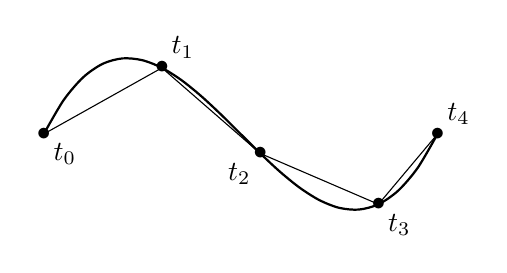
\begin{tikzpicture}[scale=2.5]
	\draw [thick] plot [smooth] coordinates {(-1,0) (-0.9, 0.171) (-0.8, 0.288) (-0.7, 0.357) (-0.6, 0.384) (-0.5, 0.375) (-0.4, 0.336) (-0.3, 0.273) (-0.2, 0.192) (-0.1, 0.099) (0,0) (0.1, -0.099) (0.2, -0.192) (0.3, -0.273) (0.4, -0.336) (0.5, -0.375) (0.6, -0.384) (0.7, -0.357) (0.8, -0.288) (0.9, -0.171) (1,0)}; %
	
	\foreach \s/\t/\u/\v in {-1/0/-0.4/0.336, -0.4/0.336/0.1/-0.099, 0.1/-0.099/0.7/-0.357, 0.7/-0.357/1/0}
	{
		\draw (\s,\t) -- (\u,\v);
		\draw (\s,\t) node {$\bullet$};
	}
	
	\draw (-1,0) node [below right] {$t_0$};
	\draw (-0.4,0.336) node [above right] {$t_1$};
	\draw (0.1,-0.099) node [below left] {$t_2$};
	\draw (0.7,-0.357) node [below right] {$t_3$};
	\draw (1,0) node [above right] {$t_4$};
	
	\draw (1,0) node {$\bullet$};
	
\end{tikzpicture}
\end{center}

Let's try to formalise this. Let $A = \left\{0 = t_0 < t_1 < \cdots < t_n = 1 \right\} \subset [0,1]$ be a finite subset. Now define
\begin{equation*}
	L_A(\gamma) = \sum_{i=1}^n d(\gamma(t_i), \gamma(t_{i-1})).
\end{equation*}
It should be clear that if we increase an extra point, $\overline{t_j}$, that this length increases.

\begin{center}
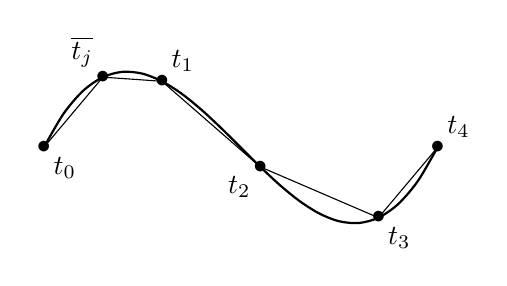
\begin{tikzpicture}[scale=2.5]
	\draw [thick] plot [smooth] coordinates {(-1,0) (-0.9, 0.171) (-0.8, 0.288) (-0.7, 0.357) (-0.6, 0.384) (-0.5, 0.375) (-0.4, 0.336) (-0.3, 0.273) (-0.2, 0.192) (-0.1, 0.099) (0,0) (0.1, -0.099) (0.2, -0.192) (0.3, -0.273) (0.4, -0.336) (0.5, -0.375) (0.6, -0.384) (0.7, -0.357) (0.8, -0.288) (0.9, -0.171) (1,0)}; %
	
	\foreach \s/\t/\u/\v in {-1/0/-0.7/0.357, -0.7/0.357/-0.4/0.336, -0.4/0.336/0.1/-0.099, 0.1/-0.099/0.7/-0.357, 0.7/-0.357/1/0}
	{
		\draw (\s,\t) -- (\u,\v);
		\draw (\s,\t) node {$\bullet$};
	}
	
	\draw (-1,0) node [below right] {$t_0$};
	\draw (-0.4,0.336) node [above right] {$t_1$};
	\draw (0.1,-0.099) node [below left] {$t_2$};
	\draw (0.7,-0.357) node [below right] {$t_3$};
	\draw (1,0) node [above right] {$t_4$};
	
	\draw (-0.7,0.357) node [above left] {$\overline{t_j}$};
	
	\draw (1,0) node {$\bullet$};
	
\end{tikzpicture}
\end{center}

If we let $A\p = \left\{ 0 = t_0 < t_1 < \cdots < t_{j-1} < \overline{t_j} < t_j < \cdots < t_n = 1 \right\}$, then by the triangle inequality, $L_{A\p}(\gamma) \geq L_A(\gamma)$. Thus:
\begin{equation*}
	L_A(\gamma) \geq L_{\{0,1\}}(\gamma) = d(\gamma(0),\gamma(1)).
\end{equation*}
Also we have that if $A \subset A\p$, then $L_A(\gamma) \leq L_{A\p}(\gamma)$.

	\pagebreak

With these thoughts, we're ready to define the length of a path, and the following definition seems natural:

\begin{definition}
	The \emph{length} of a path $\gamma$ is
	\begin{equation*}
		L(\gamma) = \sup_A L_A(\gamma)
	\end{equation*}
	as $A$ runs over the finite subsets of $[0,1]$. %
\end{definition}

\begin{example}
	The line segment from $\xx$ to $\yy$ is parameterised by $\gamma(t) = \xx + t(\yy - \xx)$.

	The triangle inequality in $\Rn$ states that
	\begin{equation*}
		\left\vert \xx - \yy \right\vert + \left\vert \yy - \zz \right\vert \geq \left\vert \xx - \zz \right\vert,
	\end{equation*}
	with equality if and only if any of the three equivalent conditions hold:
	\begin{itemize}
		\shortskip
		\item $\xx - \yy$ is a nonnegative multiple of $\yy - \zz$;
		\item $\xx - \zz$ is a $\geq 1$ multiple of $\yy - \zz$;
		\item $\yy$ lies on the line segment from $\xx$ to $\zz$.
	\end{itemize}
	In particular, this last condition means that if $\gamma$ is a line segment from $\xx$ to $\yy$, then $L_A(\gamma) = d(\xx,\yy)$ for all $A$, and so %
	\begin{equation*}
		L(\gamma) = \sup_A L_A(\gamma) = d(\xx,\yy).
	\end{equation*}
\end{example}

Now let's check that there isn't some other path with the same length as the line segment. First we need the following lemma:

\begin{lemma}
	If $\gamma\circ f$ is a reparameterisation of $\gamma$, then $L(\gamma \circ f) = L(\gamma)$. %
\end{lemma}

\begin{proof}
	We have $L_A(\gamma \circ f) = L_{f(A)}(\gamma)$. Also $L_A(\gamma \circ f) \leq \sup_A L_A(\gamma) = L(\gamma)$, and so $L(\gamma \circ f) \leq L(\gamma)$. %
	
	Similarly $\gamma= (\gamma \circ f) \circ f^{-1}$ implies $L(\gamma) = L(\gamma \circ f \circ f^{-1}) \leq L(\gamma \circ f)$. %
	
	Hence $L(\gamma) = L(\gamma \circ f)$.
\end{proof}

\begin{proposition}
	The line segment from $\xx$ to $\yy$ is the shortest path from $\xx$ to $\yy$. Precisely, if $\gamma_0$ is the line segment from $\xx$ to $\yy$ and $\gamma_1$ is a path from $\xx$ to $\yy$ with $L(\gamma_0) = L(\gamma_1) = d(\xx,\yy)$, then $\gamma_1 = \gamma_0 \circ f$, where $f:[0,1] \to [0,1]$ is continuous, and $t\geq s \implies f(t)\geq f(s)$. %
	
	% if $\gamma_0$ is the line segment and $\gamma$ is another path from $\xx$ to $\yy$, $L(\gamma_1) \geq L(\gamma_0)$ with equality if and only if $\gamma_1 = \gamma_0 \circ f$ is a reparameterisation of $\gamma_0$. %
\end{proposition}

\vspace{-6pt}

This does not imply that $f$ is invertible. We will call this property a \emph{weak reparameterisation}.

\begin{proof}
	We've already shown that $L(\gamma_1) \geq d(\xx,\yy) = L(\gamma_0)$. To have equality, we need equality everywhere in the triangle inequality. %
	
	That means that $\gamma_1(t)$ is on the line segment for all $t$. (Otherwise $L_{\{0,t,1\}}(\gamma_1) \geq d(\xx,\yy)$.

	Thus $\gamma_1(t)=\gamma_0(f(t))$ for some $f:[0,1] \to [0,1]$. Now $f(t) = \gamma_0^{-1} \circ \gamma_1(t)$ is cts.

	Suppose that $f(s) \geq f(t)$ for $t\geq s$. Then $L_{\{0,s,t,1\}}(\gamma_1) \geq d(\xx,\yy)$.

	So if $L(\gamma_1) = L(\gamma_0)$, then $t\geq s \implies f(t) \geq f(s)$, and $f$ is a bijection.
\end{proof}

	\pagebreak

\begin{proposition}
	Suppose $\gamma:[0,1] \to \Rn$ is continuously differentiable. Then %
	\begin{equation*}
		L(\gamma) = \int_0^1 \left\vert \gamma\p(t) \right\vert \dif{t}.
	\end{equation*}
\end{proposition}

\begin{proof}
	Write $\gamma\p(t) = (\gamma_1\p(t), \ldots, \gamma_n\p(t))$. Now $\gamma_i\p(t)$ is a continuous function on a compact set, so is uniformly continuous. That is, given $\epsilon>0$, there is some $\delta>0$ such that $\left\vert \gamma_i\p(t) - \gamma_i\p(s) \right\vert < \epsilon$ whenever $\left\vert t-s \right\vert<\delta$. %
	
	By the mean value theorem,
	\begin{equation*}
		\gamma_i(t) - \gamma_i(s) = \left( t-s \right) \gamma_i\p(t_i),
	\end{equation*}
	with $s\leq t_i \leq t$.  So if $\left\vert t-s \right\vert<\delta$, then
	\begin{equation*}
		\left\vert \gamma_i(t) - \gamma_i(s) - \left( t-s \right) \gamma_i\p(t) \right\vert \leq \left\vert t-s \right\vert \left\vert \gamma_i\p(t) - \gamma_i\p(t_i) \right\vert \leq \left\vert t-s \right\vert \epsilon. %
	\end{equation*}
	Then applying the triangle inequality repeatedly, we have
	\begin{equation*}
		\left\vert \gamma(t) - \gamma(s) - \left( t-s \right) \gamma\p(t) \right\vert \leq n\left\vert t-s \right\vert \epsilon. %
	\end{equation*}
	Now if $A\subset [0,1]$ satisfies $t_i - t_{i-1}<\delta$ for all $i$, then
	\begin{equation*}
		\left\vert \sum \left\vert \gamma(t_i) - \gamma(t_{i-1}) \right\vert - \sum \left( t_i-t_{i-1} \right) \left\vert \gamma\p(t_i) \right\vert \right\vert \leq ne \sum \left\vert t_i - t_{i-1} \right\vert \leq n \epsilon. %
	\end{equation*}
	Now $\sum \left( t_i-t_{i-1} \right) \left\vert \gamma\p(t_i) \right\vert$ is the right Riemann sum for $\int_0^1 \left\vert \gamma\p(t) \right\vert \dif{t}$, so if we take $A\p$ with $t_i-t_{i-1} < \delta\p < \delta$, then %
	\begin{equation*}
		\left\vert \sum \left( t_i-t_{i-1} \right) \left\vert \gamma\p(t_i) \right\vert - \int_0^1 \left\vert \gamma\p(t) \right\vert \dif{t} \right\vert \leq \epsilon. %
	\end{equation*}
	Thus we have
	\begin{equation*}
		\left\vert L_{A\p}(\gamma) - \int_0^1 \left\vert \gamma\p(t) \right\vert \dif{t} \right\vert < \left( n+1 \right) \epsilon %
	\end{equation*}
	whenever $t_i-t_{i-1} < \delta\p$ for all $i$.
	
	Given any $A$, pick $A\p$ satisfying the condiion above, then
	\begin{equation*}
		L_A(\gamma) \leq L_{A\p}(\gamma) \leq \int_0^1 \left\vert \gamma\p(t) \right\vert \dif{t} + \left( n+1 \right) \epsilon %
	\end{equation*}
	and
	\begin{equation*}
		L_{A\p}(\gamma) \geq \int_0^1 \left\vert \gamma\p(t) \right\vert \dif{t} - \left( n+1 \right)\epsilon. %
	\end{equation*}
	Combining these two, we have
	\begin{equation*}
		L(\gamma) = \sup_A L_A(\gamma) = \int_0^1 \left\vert \gamma\p(t) \right\vert \dif{t}. \qedhere %
	\end{equation*}
\end{proof}

% subsection geometry_in_rn (end)

	\pagebreak

\subsection[Isometries of $\Rn$]{Isometries of $\boldsymbol{\sf{R}^\sf{n}}$} % (fold)
\label{sub:isometries_of_rn}

\begin{definition}
	Let $(X,d_X)$ and $(Y,d_Y)$ be metric spaces. A bijection $\phi:X\to Y$ is an \emph{isometry} if it preserves distances; that is, %
	\begin{equation*}
		d_X(X_1,X_2) = d_Y(\phi(X_1), \phi(X_2))
	\end{equation*}
	for all $X_1, X_2 \in X$.
\end{definition}

An isometry is continuous: given $\epsilon>0$, $d_Y(\phi(X_1),\phi(X_2)) < \epsilon$ whenever $d_X(X_1,X_2) < \epsilon$.

\begin{lemma}
	The inverse of an isometry is an isometry. The composition of two isometries is an isometry. %
\end{lemma}

\begin{proof}
	Suppose $\phi:X \to Y$ is an isometry with $\phi(X_i) = Y_i$. Then $d_Y(Y_1, Y_2) = d_X(X_1,X_2)$, and so $d_Y(Y_1,Y_2) = d_X(\phi^{-1}(Y_1), \phi^{-1}(Y_2))$, which shows that $\phi^{-1}$ is an isometry. %
	
	If $\psi: Y \to Z$ is an isometry, then
	\begin{equation*}
		d_Z(\psi(\phi(X_1)), \psi(\phi(X_2)) = d_Y(\phi(X_1), \phi(X_2)) = d_X(X_1,X_2),
	\end{equation*}
	and so $\psi \circ \phi$ is an isometry.
\end{proof}

\begin{corollary}
	Let $\Isom(X)$ be the set of isometries:
	\begin{equation*}
		\Isom(X) = \left\{\phi:X \to X \mid \phi \text{ is an isometry}\right\}.
	\end{equation*}
	Then $\Isom(X)$ is a group under composition. %
\end{corollary}

\lecturemarker{3}{28 Jan}

\begin{examples}
\mbox{}
\begin{enumerate}
	\item \emph{Translations.} If $\vv\iRn$, define $T_{\vv}:\Rn\to\Rn$ by $T_{\vv}(\xx) = \xx + \vv$. Then %
	\begin{equation*}
		\left\vert T_{\vv}(\xx) - T_{\vv}(\yy) \right\vert
		= \left\vert \xx+\vv - \yy-\vv \right\vert
		= \left\vert \xx-\yy \right\vert.
	\end{equation*}
	It is clear that $T_{\vv}$ is bijective by $T_{\vv}^{-1} = T_{-\vv}$, and hence $T_{\vv}$ is an isometry. %
	
	\item \emph{Orthogonal transformations.} Recall that a \emph{linear} map $O:\Rn\to\Rn$ is orthogonal if
	\begin{equation*}
		O(\vv) \cdot O(\ww) = \vv \cdot \ww
	\end{equation*}
	for all $\vv,\ww \iRn$. (Or in matrix form, $OO^\Trans = I$.) The set of all such transformations is the \emph{orthogonal group}, $O(n)$. If $O\in O(n)$, then
	\begin{equation*}
		O\vv \cdot O\vv = \vv \cdot \vv \implies \left\vert O\vv \right\vert = \left\vert \vv \right\vert.
	\end{equation*}
	Then using the fact that $O\in O(n)$ is a linear map:
	\begin{equation*}
		\left\vert O\xx - O\yy \right\vert = \left\vert O\left( \xx-\yy \right) \right\vert = \left\vert \xx-\yy \right\vert, %
	\end{equation*}
	and so $O$ is an isometry.
	
	Consider the case $n=2$. $O\in O(2)$ looks like
	\begin{equation*}
		\mat{\cos\theta & -\sin\theta \\ \sin\theta & \cos\theta},
	\end{equation*}
	rotation by an angle $\theta$ around the origin.
	
		\pagebreak
	
	\begin{center}
	\begin{tikzpicture}[scale=2.5]
		
		\draw (0,-0.2) -- (0,1.2);
		\draw (-1.2,0) -- (1.2,0);
		
		\bigarrow (0,0) -- (1,0) node [below right] {$\ee_1$};
		\bigarrow (0,0) -- (0,1) node [right] {$\ee_2$};
		
		\bigarrow (0,0) -- (0.866,0.5) node [right] {$O(\ee_1) = (\cos\theta,\sin\theta)$};
		\bigarrow (0,0) -- (-0.5,0.866) node [left] {$=(\cos(\theta+\f{\pi}{2}),\sin(\theta+\f{\pi}{2}))$};
		\draw (-0.72,1.066) node [left] {$O(\ee_2) = (-\sin\theta,\cos\theta) \hspace{1cm}$};

		% 0.15
		
		\draw (0.0866,0.05) -- (0.0366,0.1366) -- (-0.05,0.0866);
		
		\draw (0.35,0) arc (0:30:0.35);
		\draw (0.33,0.11) node [right] {$\theta$};
		
	\end{tikzpicture}
	\end{center}
	or like
	\begin{equation*}
		\mat{\cos\theta & \phantom{-}\sin\theta \\ \sin\theta & -\cos\theta},
	\end{equation*}
	reflection in the line that makes angle $\theta/2$ with the $x$-axis.
	
	\emph{Proof.}
	\begin{equation*}
		\mat{\cos\theta & \sin\theta \\ \sin\theta & -\cos\theta}
		= \underset{\text{rotate by $\theta/2$}}{\mat{\cos\theta/2 & -\sin\theta/2 \\ \sin\theta/2 & \phantom{-}\cos\theta/2}} %
		  \underset{\substack{\text{reflect across} \\ \text{$x$-axis}}}{\mat{1 & 0 \\ 0 & -1}}
		  \underset{\text{rotate by }-\theta/2}{\mat{\phantom{-}\cos\theta/2 & \sin\theta/2 \\ -\sin\theta/2 & \cos\theta/2}}. %
	\end{equation*}
	How do we tell these two apart? We note that rotations have determinant $+1$, whereas reflections have determinant $-1$.
	
	\item \emph{Rotation by angle $\theta$ about some $\pp\iRn$.}
	Here we translate $\pp\iRn$ to the origin, perform our rotation, then undo the translation. That is, we have the composition $\phi=T_{\pp} \circ O_\theta \circ T_{-\pp}$, or %
	\begin{equation*}
		\phi(\xx) = \pp + O\left( \xx-\pp \right) = O\xx + \left( \pp-\theta\pp \right).
	\end{equation*}
\end{enumerate}
\end{examples}

It turns out that these examples are all we need to generate the orthogonal group, which is summarised by the following theorem:

\begin{theorem}
	Every $\phi\in\Isom(\Rn)$ can be written as $\phi=T_{\vv} \circ O$ for some $\vv\iRn$ and $O\in O(n)$; that is, $\phi(\xx)=O(\xx) + \vv$. %
\end{theorem}

We will prove this theorem through a series of lemmas.

\begin{lemma}
	\label{lem:orthog-1} If $\phi\in\Isom(\Rn)$ satisfies $\phi(\OO) = \OO$ and $\phi(\ee_i) = \ee_i$, where $\{\ee_i\}$ is the standard basis, then $\phi=\id_{\Rn}$. %
\end{lemma}

\begin{proof}
	Let $\phi(\xx)=\yy$. Then
	\begin{equation*}
		\vert \xx-\OO \vert^2
		= \vert \phi(\xx) - \phi(\OO) \vert^2
		= \vert \phi(\xx)-\OO \vert^2
		= \vert \yy \vert^2,
	\end{equation*}
	and so we have
	\begin{equation*}
		\textstyle\sum_{i=1}^n x_i^2 = \sum_{i=1}^n y_i^2. \tag{$*$}
		\label{eq:orthog-lem-11}
	\end{equation*}
	Similarly, for any basis vector $\ee_i$, we have
	\begin{equation*}
		\left\vert \xx-\ee_i \right\vert^2
		= \left\vert \phi(\xx) - \phi(\ee_i) \right\vert^2
		= \left\vert \yy - \ee_i \right\vert^2.
	\end{equation*}
	Hence we have
	\begin{equation*}
		x_1^2 + x_2^2 + \cdots + (x_i-1)^2 + \cdots + x_n^2 = y_1^2 + y_2^2 + \cdots + (y_i-1)^2 + \cdots + y_n^2. %
		\tag{$**$}
		\label{eq:orthog-lem-12}
	\end{equation*}
	Subtracting \eqref{eq:orthog-lem-11} from \eqref{eq:orthog-lem-12} gives $-2x_i+1 = -2y_i+1 \implies x_i=y_i$. Hence $\yy=\xx$, and $\phi=\id_{\Rn}$. %
\end{proof}

\begin{lemma}
	\label{lem:orthog-2} If $\phi\in\Isom(\Rn)$ satisfies $\phi(\OO) = \OO$, then $\phi(\xx) \cdot \phi(\yy) = \xx\cdot\yy$ for all $\xx,\yy\iRn$. %
\end{lemma}

\begin{proof}
	First we have
	\begin{equation*}
		\left\vert \phi(\xx) \right\vert^2
		= \left\vert \phi(\xx)-\phi(\OO) \right\vert^2
		= \left\vert \xx-\OO \right\vert^2
		= \left\vert \xx \right\vert^2.
		\tag{$*$}
		\label{eq:orthog-lem-21}
	\end{equation*}
	We also have
	\begin{equation*}
		\left\vert \phi(\xx)-\phi(\yy) \right\vert^2 = \left\vert \xx-\yy \right\vert^2.
	\end{equation*}
	This is also equal to
	\begin{equation*}
		\left\vert \phi(\xx) \right\vert^2 - 2\,\phi(\xx) \cdot \phi(\yy) + \left\vert \phi(\yy) \right\vert^2
		= \left\vert \xx \right\vert^2 - 2\,\xx\cdot\yy + \left\vert \yy \right\vert^2.
	\end{equation*}
	Finally, using \eqref{eq:orthog-lem-21}, we get $\phi(\xx)\cdot\phi(\yy) = \xx\cdot\yy$. %
\end{proof}

\begin{lemma}
	\label{lem:orthog-3} If $\phi\in\Isom(\Rn)$ with $\phi(\OO)=\OO$, then $\phi(\xx) = O\xx$ for some $O\in O(n)$. %
\end{lemma}

\begin{proof}
	Let $\vv_i=\phi(\ee_i)$. Then $\vv_i\cdot\vv_j = \phi(\ee_i) \cdot \phi(\ee_j) = \ee_i \cdot \ee_j = \delta_{ij}$ (lemma~\ref{lem:orthog-2}). %

	Thus $O=(\vv_1,\ldots,\vv_n) \in O(n)$, with $O(\ee_i)=\vv_i$.

	Then $O^{-1}\circ\phi\in\Isom(\Rn)$, and by lemma~\ref{lem:orthog-1},
	\begin{equation*}
		\begin{rcases}
			& O^{-1}\circ\phi(\ee_i) = \ee_i \\
			& O^{-1}\circ\phi(\OO) = \OO
		\end{rcases}
		\implies O^{-1}\circ \phi=\textstyle \id_{\Rn}
	\end{equation*}
	and so we have $\phi=O$. %
\end{proof}

\begin{proof}
	[Proof of theorem] Let $\vv = \phi(\OO)$. Then by lemma~\ref{lem:orthog-3},
	\begin{equation*}
		T_{\vv}^{-1} \circ \phi(\OO) = \OO, \qquad
		T_{\vv}^{-1} \circ \phi(\xx) = O\xx.
	\end{equation*}
	Thus $\phi(\xx)=O\xx+\vv$. %
\end{proof}

\begin{corollary}
	Isometries preserve angles. That is, if $\phi\in\Isom(\Rn)$, and $R_1,R_2$ are rays starting at $\xx$, then $\angle\phi(R_1),\phi(R_2) = \angle R_1,R_2$. %
\end{corollary}

\begin{proof}
	It suffices to check for $\phi=T_{\vv}$ and $\phi=O$. If $R_i$ has direction vector $\vv_i$, then
	\begin{equation*}
		T_{\vv}(R_i)
		= T_{\vv}\left( \left\{\xx+t\vv_i \mid t\geq 0 \right\} \right)
		= \left\{\vv_i+\xx+t\vv_i \mid t\geq 0 \right\}
	\end{equation*}
	which has direction vector $\vv_i$ also and so the angle is unchanged.

	Similarly $OR_i$ has direction vector $O\vv_i$, and we know that
	\begin{equation*}
		O\vv_1 \cdot O\vv_2 = \vv_1 \cdot \vv_2,
	\end{equation*}
	and so the angle is unchanged.
\end{proof}

	\pagebreak

\begin{definition}
	An \emph{orthogonal frame} at $\xx$ is an $n$-tuple of perpendicular rays, denoted $(R_1,\ldots,R_n)$, starting at $X$. %
	
	The \emph{standard frame} is $F_0=(X_1,\ldots,X_n)$, where $X_i$ is the positive $x_i$-axis. %
\end{definition}

\begin{corollary} % Corollary 2 
	If $F_1$ and $F_2$ are orthogonal frames, then there is a unique $\phi\in\Isom(\Rn)$ with $\phi(F_1)=F_2$. %
\end{corollary}

\begin{proof}
	Let $\vv_i^j$ be the direction vector for $R_i$. Then %
	\begin{equation*}
		O = \left( \f{\vv_1^j}{\Vert \vv_1^j \Vert}, \ldots, \f{\vv_n^j}{\Vert \vv_n^j \Vert} \right) \in O(n).
	\end{equation*}
	Let $\phi_j = T_{\xx_j} \circ O_j$ and $F_j = (R_1^j, \ldots, R_n^j)$.
	
	Then $\phi_j(F_0) = F_j$, and so $\phi=\phi_2\circ\phi^{-1}$ has
	\begin{equation*}
		\phi(F_1) =\phi_2(\phi_1^{-1}(F_1)) = \phi_2(F_0) = F_2.
	\end{equation*}
	That proves existence, now for uniqueness: if $\phi\p(F_1) = F_2$, then
	\begin{equation*}
		\phi_2^{-1} \circ \phi\p \circ \phi_1(F_0) = \phi_2^{-1}(\phi(F_1)) = \phi_2^{-1}(F_2) = F_0,
	\end{equation*}
	and $\phi_2^{-1} \circ \phi\p \circ \phi_1 = \id_{\Rn}$ by lemma~\ref{lem:orthog-1}. Thus $\phi\p = \phi_2 \circ \phi_1^{-1} = \phi$. %
\end{proof}

% subsection isometries_of_rn (end)

\subsection{The Euclidean plane} \lecturemarker{4}{30 Jan} % (fold)
\label{sub:the_euclidean_plane}

\begin{proposition}
	Two distinct lines in $\R^2$ intersect in at most one point. %
\end{proposition}

\begin{proof}
	The intersections are solutions of
	\begin{equation*}
		\xx+t\vv_1 = \yy+s\vv_2.
	\end{equation*}
	Rearranging this, we have
	\begin{equation*}
		t\vv_1 - s\vv_2 = \yy-\xx.
	\end{equation*}
	If $\vv_1$ and $\vv_2$ are linearly independent, then there is a unique solution. If they are linearly dependent:
	\begin{itemize}
		\shortskip
		\item either $\yy-\xx$ is in the span of $\vv_1$, and the lines are the same;
		\item or $\yy-\xx$ is not in the span of $\vv_1$, and there are no solutions. \qedhere
	\end{itemize}
\end{proof}

\begin{definition}
	Two distinct lines in $\R^2$ are \emph{parallel} if they do not intersect. %
\end{definition}

\begin{corollary}
	If $L$ is a line, and $p$ is a point not on $L$, then there is a unique line $L\p$, that passes through $p$ and is parallel to $L$. %
\end{corollary}

\begin{proof}
	The calculation above shows that the direction vector of $L\p$ is a scalar multiple of the direction vector of $L$.

	We saw before that there's a unique line passing through $p$ with a given diection (up to scalar multiple). %
\end{proof}

\begin{definition}
	The \emph{circle of radius $r$, centred at $\xx$} is given by
	\begin{equation*}
		\left\{ \yy : d(\xx,\yy) = r\right\}.
	\end{equation*}
\end{definition}

\begin{proposition}
	A line and a circle intersect in at most two points. %
\end{proposition}

\begin{proof}
	Suppose the circle is centred at $p$.

	We need to solve the two equations:
	\begin{gather*}
		ax_1 + bx_2 + c = 0, \tag{line} \\
		\left( x_1-p_1 \right)^2 + \left( x_2-p_2 \right)^2 = r^2. \tag{circle}
	\end{gather*}
	We can solve for $x_1$ in terms of $x_2$ (or vice versa, if $a=0$). Substitute to get a quadratic equation for $x_2$, and so there are at most two solutions. %
\end{proof}

% subsection the_euclidean_plane (end)